\documentclass[resume]{subfiles}


\begin{document}
\section{Firewall iptables}
Il est nécessaire d'activer netfilter dans la configuration du kernel. Un hook est une étape lors du passage d'une trame dans le stack de protocoles. Le framework netfilter sera appelé à chaque hook
\begin{figure}[H]
\centering
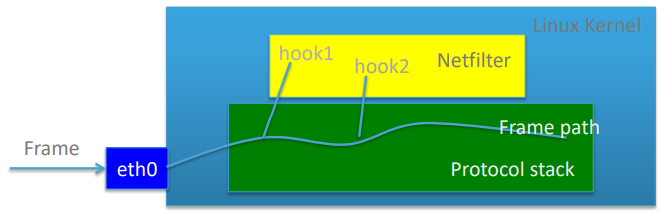
\includegraphics[width=0.75\columnwidth]{img_6.png}
\end{figure}
On peut configurer netfilter avec la commande \verb!iptables!. \verb!ebtables! permet de configurer la couche 2 uniquement (Linux bridge). \verb!nftables! vise à remplacer tout le framework
\begin{figure}[H]
\centering
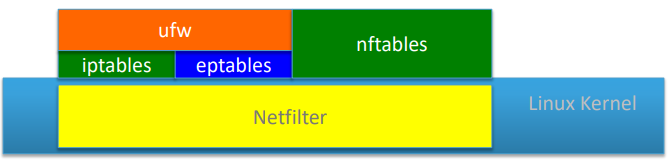
\includegraphics[width=0.5\columnwidth]{img_7.png}
\end{figure}
\subsection{Features}
\begin{enumerate}
\item Stateless packet filtering (table filter et ACCEPT, DROP, REJECT)
\item Stateful packet filtering
\item Translation d'adresses / ports
\item API pour autres applications
\end{enumerate}
\subsection{Chain}
la combinaison Chain-Table constitue les hooks
\paragraph{Chains} : INPUT, OUTPUT, FORWARD, PREROUTING, POSTROUTING
\subsubsection{Tables}
\begin{itemize}
\item raw
\item mangle (modification spéciales sur des paquets)
\item nat (consultée lorsqu'un paquet créé une nouvelle connexion)
\item filter (table de base)
\end{itemize}
\begin{figure}[H]
\centering
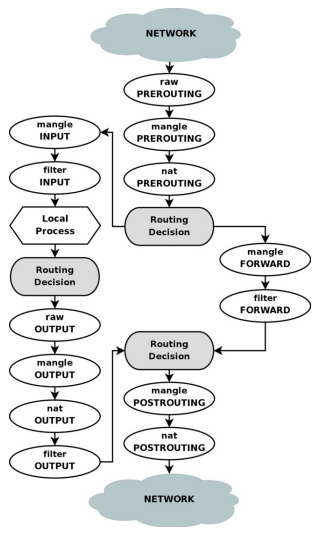
\includegraphics[width=3.50cm]{img_8.png}
\end{figure}
\subsection{Commande iptables}
\begin{center}
\verb!iptables -t table -COMMAND chain ... -j TARGET!
\end{center}

\end{document}